\documentclass{thesisbeamer}

\usepackage{caption}
\usepackage{comment}
\usepackage{amsmath}
\usepackage{bm}
\usepackage{multicol}
\usepackage{xcolor}
\usepackage{tabularx}
\usepackage{optidef}
\usepackage{mathtools}

\usepackage{comment}
\usepackage{graphicx}
\usepackage{subcaption}
\captionsetup{compatibility=false}

\title[Making Flips with Quadrotors in Constrained Environments]{Making Flips with Quadrotors in Constrained Environments}
\author[Elie Hatem]{Elie Hatem \newline ~ \newline \normalsize{Advisors: Dr. Sebastien Briot, Dr. Isabelle Fantoni}}
\date{\today}

\setbeamerfont{caption}{size=\tiny}

\newcommand\Fontvi{\fontsize{9}{10}\selectfont}


\bibliography{../biblio}

% video will work on Linux (with Okular) or OS X, for other OS's or viewers find your own way to do it
%\videoOSX	% for OS X 
\videoOFF

\AtBeginSection[]
{
     \begin{frame}[allowframebreaks]
         \frametitle{Table of Contents}
         \tableofcontents[currentsection]
     \end{frame}
}

\begin{document}

\MakeTitleNoFoot

\begin{frame}[allowframebreaks]
	\frametitle{Table of Contents}
     \tableofcontents
\end{frame}


\section{Introduction}

\begin{frame}
\frametitle{The Quatrotor Platform}
\Fontvi

\begin{figure}[t]
     \centering
     \begin{subfigure}[b]{0.45\textwidth}
         \centering
         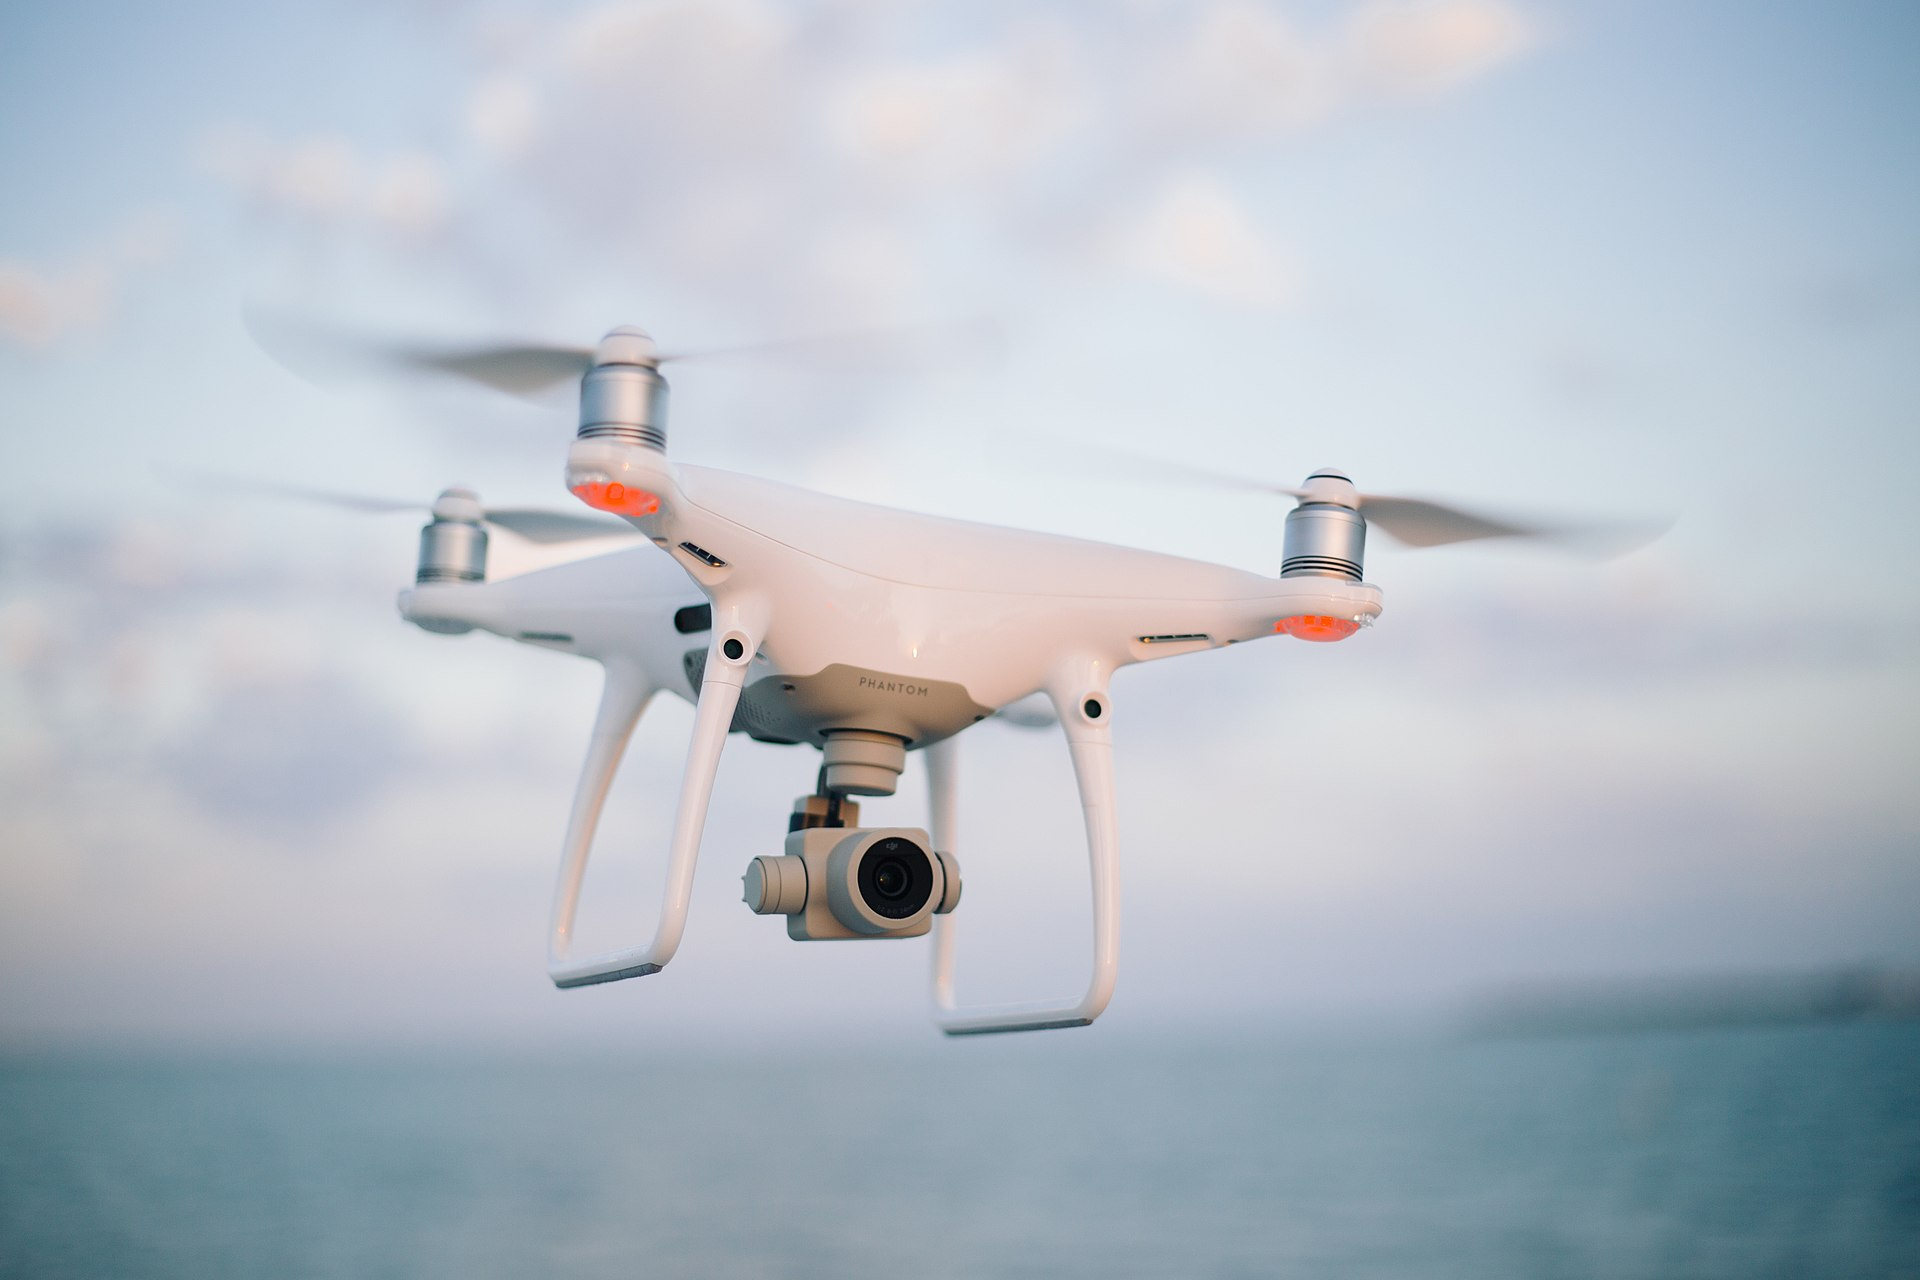
\includegraphics[width=\textwidth]{Images/Introduction/drone}
         \caption[Caption for LOF]{DJI Phantom quadcopter (UAV)\protect\footnotemark}
         \label{fig:drone}
     \end{subfigure}
     \hfill
     \begin{subfigure}[b]{0.45\textwidth}
         \centering
         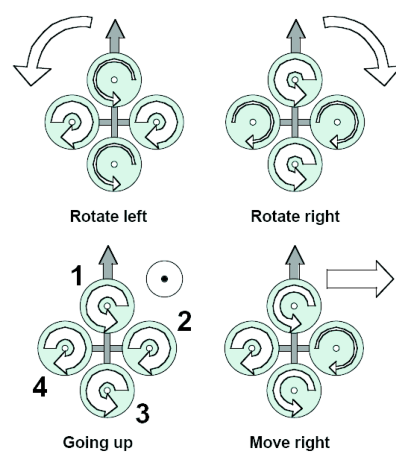
\includegraphics[width=0.6\textwidth]{Images/Introduction/propeller_direction.svg}
         \caption{Quadrotor Concept. Width of the arrows is proportional to the angular speed of the propellers\protect\footnotemark}
         \label{fig:propeller_directions}
     \end{subfigure}
        \caption{Commercial quadrtotor platform (left) and quadrotor concept (right).}
        \label{fig:three graphs}
\end{figure}

\footnotetext[1]{\tiny{\url{https://en.wikipedia.org/wiki/Quadcopter\#/media/File:Quadcopter_camera_drone_in_flight.jpg}}}
\footnotetext[2]{\tiny{Design and control of quadrotors with application to autonomous flying, 2007, S. Bouabdallah}}

\end{frame}


\begin{frame}
\frametitle{The Quatrotor Platform}
\Fontvi

Over the last few years, quadrotors have gained large popularity in academia and industry. Because, they are:

\begin{itemize}
	\item Simple to design and assemble using relatively cheap components.
	\item Different use cases: aerial photography, agriculture, surveillance tasks, etc.
	\item Quite agile and maneuverable during flight, especially when compared to other types of UAVs.
\end{itemize}

\end{frame}

\begin{frame}
\frametitle{Main Challenges}
\Fontvi

\begin{block}{One of the main challenges}
	Designing control and planning methods to allow tracking aggressive trajectories.
\end{block}

This difficulty is due to: 
\begin{itemize}
	\item The fast dynamics associated with the small dimensions of such agile quadrotors.
	\item Several dynamic effects will become important to consider during aggressive flight maneuvers.
	\item The motors will be commanded high speeds and accelerations, which will cause them to saturate and introduce delays.
\end{itemize}


\end{frame}



\begin{frame}
\frametitle{Goals of the Master Thesis}
\Fontvi

The goals of the master thesis: 

\begin{itemize} % [<+->]
	\item Study of multi-flip maneuvers.
	\item Implement Model Predictive Control to solve the presented issues.
	\item Perform the maneuvers in a constrained environment.
\end{itemize}

\begin{figure}[h]
     \centering
     \begin{subfigure}[h]{0.4\textwidth}
         \centering
         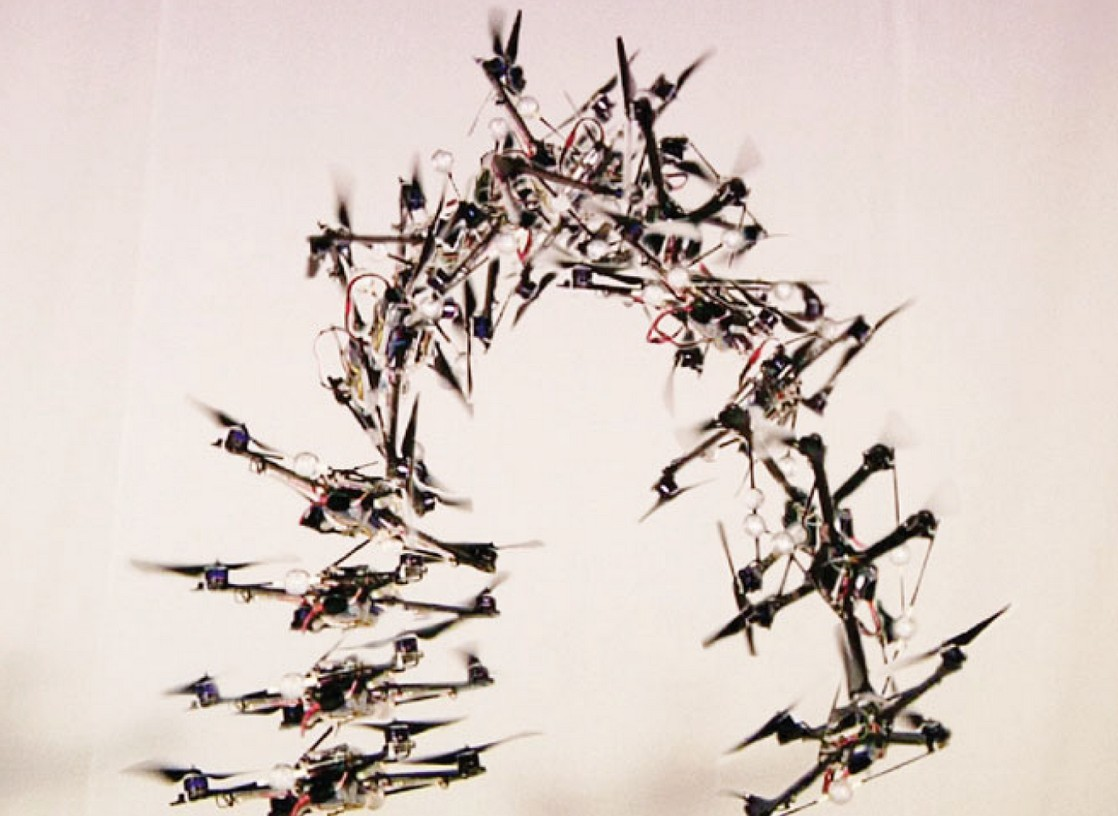
\includegraphics[width=0.9\textwidth]{Images/Introduction/flip}
    \caption{Quadrotor performing a triple flip\protect\footnotemark}
         \label{triple_flip}
     \end{subfigure}
     \hfill
     \begin{subfigure}[h]{0.38\textwidth}
         \centering
         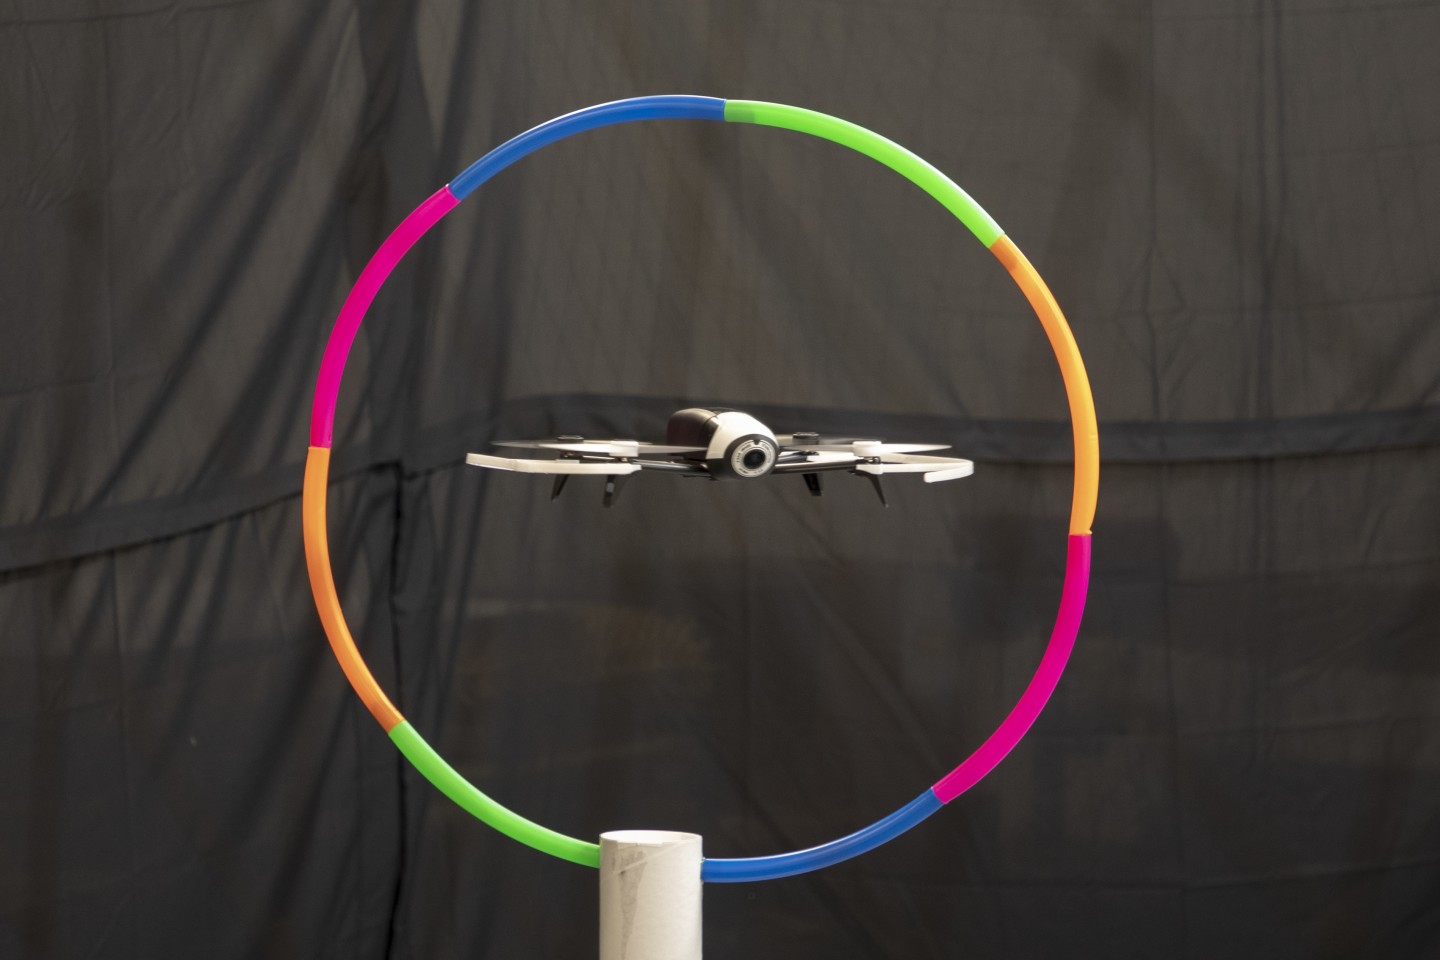
\includegraphics[width=\textwidth]{Images/Introduction/constrained_environment}
         \caption[Caption for LOF]{Quadrotor going though a loop\protect\footnotemark}
         \label{drone_hulahoop}
     \end{subfigure}
        \caption{\tiny{Representation of the issues to be tackled in this master thesis.}}
        \label{fig:three graphs}
\end{figure}

\footnotetext[3]{\tiny{Adaptive fast open-loop maneuvers for quadrocopters, 2012, S. Lupashin and R. D’Andrea}}
\footnotetext[4]{\tiny{ \url{https://newatlas.com/drones/muscle-signals-drone-control/} }}

\end{frame}

\begin{frame}
\frametitle{General Control Architecture of a Quadrotor}

	\Fontvi	
		
	\begin{figure}
		\centering
		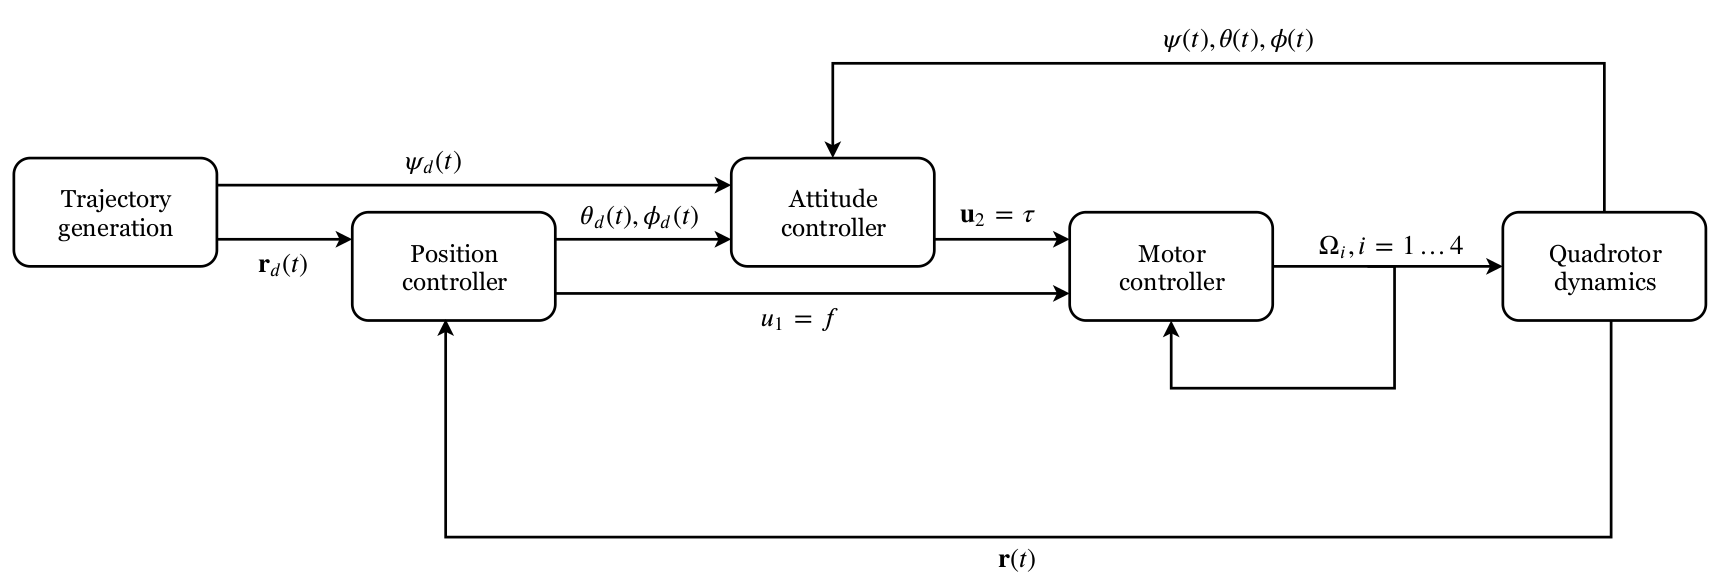
\includegraphics[width=0.9\textwidth]{diagrams/general_control_architecture.png}
		\caption{Diagram of the general control architecture of a quadrotor.}
	\end{figure}
	\begin{itemize} % [<+->]
		\item Position controller: slow rise time - drives translational dynamics errors to 0.
		\item Attitude controller: faster rise time - drives rotational dynamics errors to 0.
		\item Motor controller: fastest rise time - maps the control inputs to motor speeds.
	\end{itemize}
	\begingroup
    \fontsize{9pt}{10pt}\selectfont
    \begin{alertblock}{Remark}
		\begin{itemize}
			\item The designed controller cannot be faster than the one at a lower level.
				\begin{itemize}
					\item \fontsize{9pt}{10pt}\selectfont The orientation cannot be controlled any faster than the motors can be controlled.
				\end{itemize}
		\end{itemize}
		\end{alertblock}
\endgroup						
\end{frame}



\begin{frame}
	\frametitle{Differential Flatness}
	\Fontvi	

	A well-established finding is that the dynamic model of a quadrotor is differentially flat:
	\begin{itemize}
		\item The system with state $\bm{x} \in \mathbb{R}^n$ and input $\bm{u} \in \mathbb{R}^m$ has flat outputs $\bm{y} \in \mathbb{R}^m$ which have the following form:
	
	\begin{equation}
 \textbf{y} = \textbf{y}(\textbf{x}, \textbf{u}, \dot{\textbf{u}},...,\textbf{u}^{(p)})
 \end{equation}

 With, 
 
 \begin{equation}
 	\begin{cases}
 		\textbf{\textsc{x}} = \textbf{x}(\textbf{y}, \dot{\textbf{y}},...,\textbf{y}^{(q)}) \\
 	\\
 		\textbf{u} = \textbf{u}(\textbf{y}, \dot{\textbf{y}},...,\textbf{y}^{(r)}) \\
 	\end{cases}
 \end{equation}	
	
	
	 \item Very useful property in under-actuated systems where $m<n$.
	 \item Allows to generate trajectories in the lower dimensional space $m$.
	 \item The trajectories can then be mapped into the full dimensional space $n$.
	\end{itemize}

\end{frame}


\begin{frame}
	\frametitle{Differential Flatness}
	\Fontvi
	
	The standard choice of flat outputs for the quadrotor are:

\begin{equation}\label{flat_outputs}
\textbf{y} = \begin{bmatrix}
x && y && z && \psi \\
\end{bmatrix}^{\intercal}
\end{equation}

As a result:
\begin{itemize}
	\item Trajectories can be designed in the 4-dimensional space.
	\item They can then be mapped to the 6-dimenstional space.
	\begin{itemize}
		\item This is due to the fact that the rotational and translational dynamics are tightly coupled.
	\end{itemize}			
\end{itemize}

\end{frame}

\section{Model Predictive Control}

\begin{frame}
	\frametitle{Model Predictive Control}
	\Fontvi	

	General idea of MPC:
 	\begin{figure}[t]
 		\centering
 		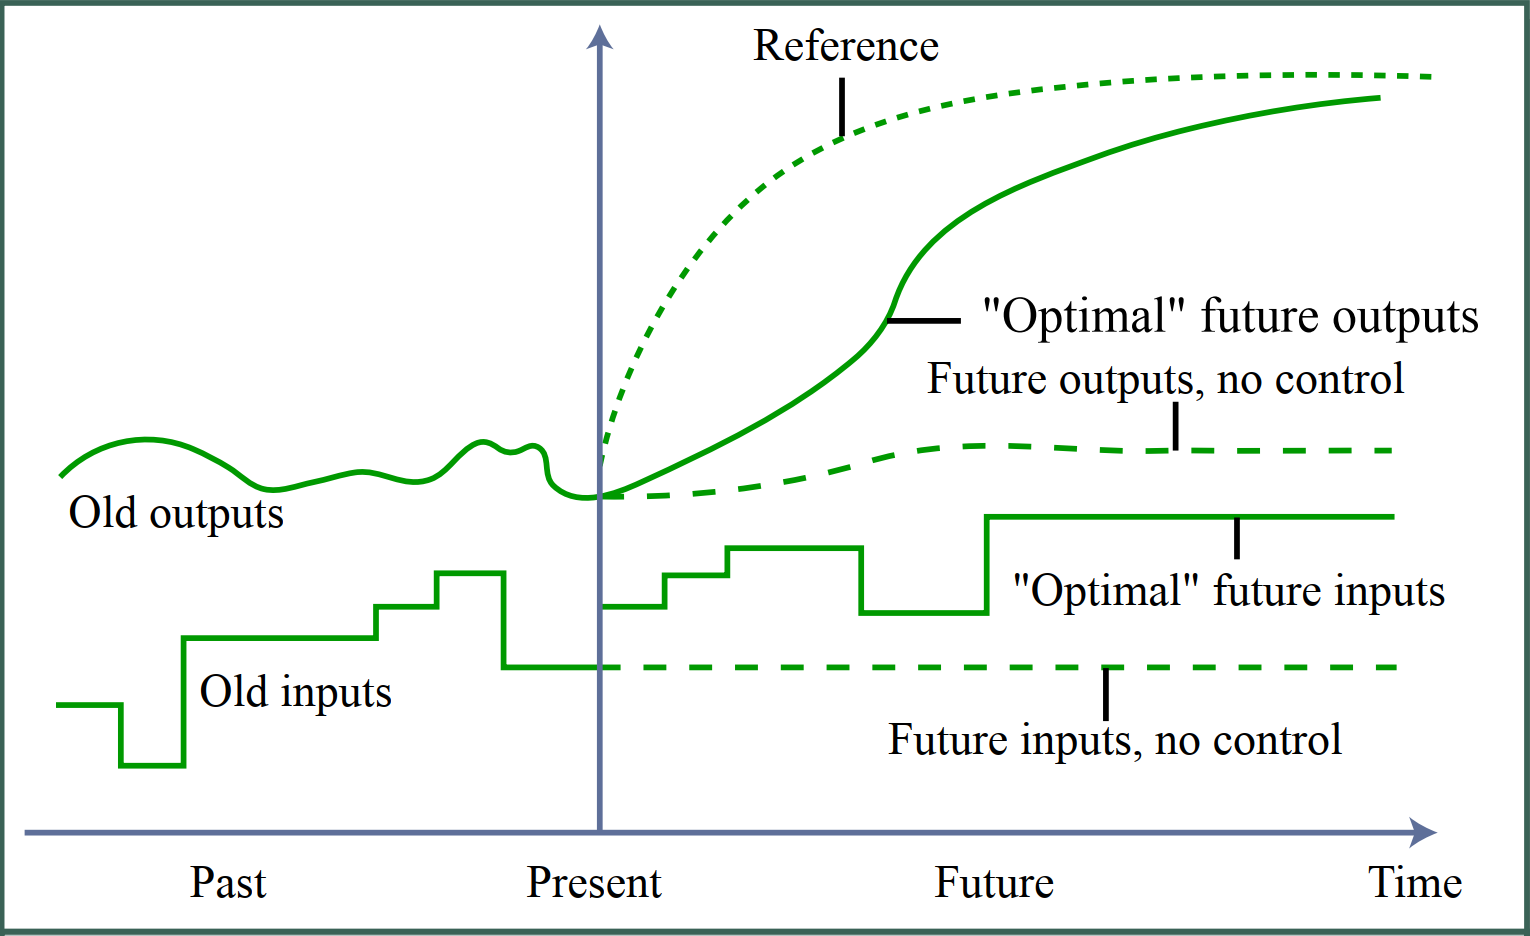
\includegraphics[width=0.5\textwidth]{Images/Control/MPC_general_idea.png}
 		\caption{Basic idea of MPC\protect\footnotemark}
 		\label{MPC_basic_idea}
	\end{figure}  

	\begin{itemize} % [<+->]
		\item It is a \textbf{feedback control} algorithm.
		\item It uses a model to \textbf{predict} future outputs.
		\item It \textbf{solves an online optimization problem} to select the optimal control.
	\end{itemize}

\footnotetext[5]{\tiny{Principles of Optimal Control, 2008, J. How}}

\end{frame}


\begin{frame}
\frametitle{Model Predictive Control}
\Fontvi	

\begin{columns}
\column {0.5\textwidth}
MPC Design parameters:

\begin{itemize} % [<+->]
	\item Sample time.
	\item Prediction horizon.
	\item Control horizon.
	\item Constraints.
	\item Weights.
\end{itemize}\pause


\column {0.5\textwidth}
Choosing proper values for these parameters is important as they affect: 
\begin{itemize}
	\item The controller performance.
	\item The computational complexity of the MPC algorithm.
\end{itemize} 
\end{columns}

\end{frame}



\begin{frame}{MPC applied on quadrotors}
\Fontvi

The most popular uses for MPC in quadrotors are:

\begin{itemize} % [<+->]
	\item Centralized MPC: Single control loop for the system.
	\item Non-centralized MPC: Cascaded control consisting of more than 1 control loop. Examples:
		\begin{itemize}
			\item MPC$_{master}$-MPC$_{slave}$
			\item MPC-PD-P
			\item Other options can be used for the inner loop.
		\end{itemize}
\end{itemize}

\begin{block}{Remark}
\begin{itemize}
	\item Centralized MPC: More accurate, high computation cost.
	\item Non-centralized MPC: Less accurate, lower computation cost. 
\end{itemize}
\end{block}

\end{frame}


\begin{frame}{Centralized MPC}
	\Fontvi

	\begin{columns}
		\begin{column}{0.5\textwidth}
			\begin{figure}
				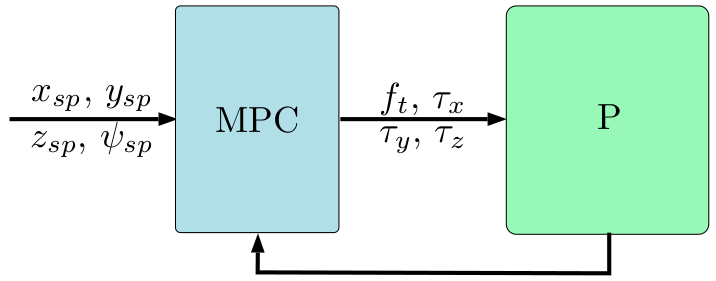
\includegraphics[width=\textwidth]{Images/Control/centralized_mpc.png}
				\caption{Centralized MPC}
			\end{figure}
		\end{column}
		\begin{column}{0.5\textwidth}
			Inputs of centralized MPC:
			\begin{itemize}
				\item Desired $x$, $y$ and $z$ positions and the yaw angle $\psi$.
			\end{itemize}
			Outputs of centralized MPC:
			\begin{itemize}
				\item Total thrust $f_t$.
				\item Torques: $\tau_x$, $\tau_y$ and $\tau_z$
			\end{itemize}
		\end{column}
	\end{columns}
	\vspace{1cm}
	Another version of the centralized MPC exists with:
	\begin{itemize}
		\item Added $\phi$ and $\theta$ angles as outputs.
	\end{itemize}
\end{frame}

\begin{frame}{Non-centralized MPC}
	\Fontvi

			\begin{figure}
				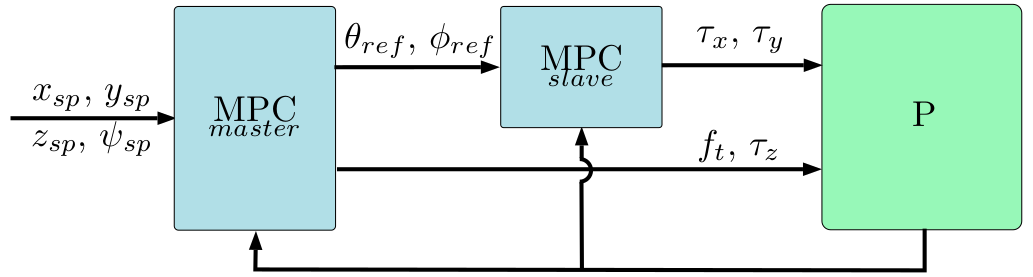
\includegraphics[width=0.7\textwidth]{Images/Control/non-centralized_mpc_1.png}
				\caption{Non-centralized MPC (MPC$_{master}$-MPC$_{slave}$)}
			\end{figure}

			Outer-loop: master MPC
			\begin{itemize}
				\item Inputs: Desired $x$, $y$, $z$, $\psi$.
				\item Outputs: $f_t$, $\tau_z$, $\theta_{ref}$, $\phi_{ref}$.
			\end{itemize}
			Inner-loop: slave MPC
			\begin{itemize}
				\item Inputs: $\theta_{ref}$, $\phi_{ref}$. 
				\item Outputs: $\tau_x$, $\tau_y$.
			\end{itemize}

\end{frame}

\begin{frame}{Non-centralized MPC}
	\Fontvi
	
			\begin{figure}
				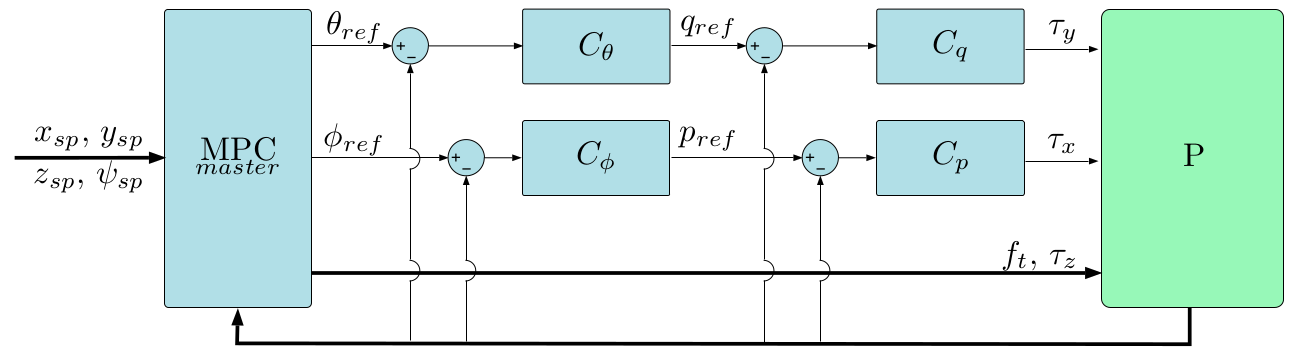
\includegraphics[width=0.7\textwidth]{Images/Control/non-centralized_mpc_2.png}
				\caption{Non-centralized MPC (MPC-PD-P)}
			\end{figure}
			Outer-loop: master MPC
			\begin{itemize}
				\item Inputs: Desired $x$, $y$, $z$, $\psi$.
				\item Outputs: $f_t$, $\tau_z$, $\theta_{ref}$, $\phi_{ref}$ 
			\end{itemize}
			Inner-loop: PD-P controller
			\begin{itemize}
				\item Inputs: $\theta_{ref}$, $\phi_{ref}$. 
				\item Outputs: $\tau_x$, $\tau_y$.
			\end{itemize}
\end{frame}

\begin{frame}[t]{Non-centralized MPC}
	\Fontvi
	Another example of a non-centralized MPC:
	\begin{figure}
		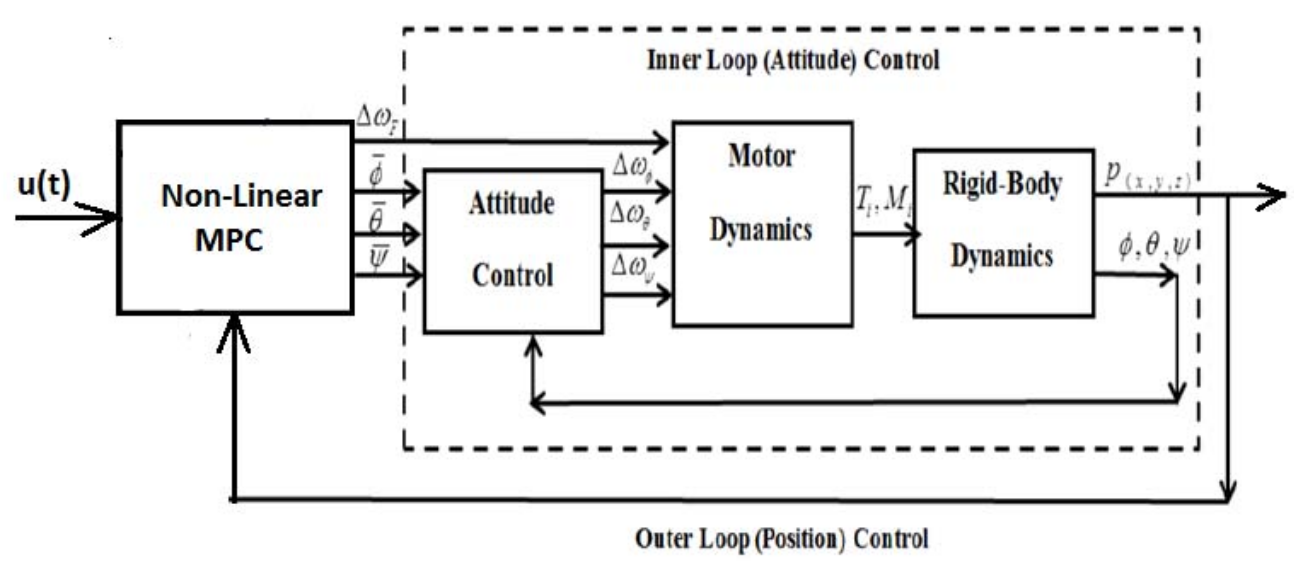
\includegraphics[width=0.7\textwidth]{Images/Control/non-centralized_mpc_3.png}
				\caption{Non-centralized MPC}
	\end{figure}
	\begin{alertblock}{Remark}
	 	The inner-loop can remain fixed, while the outer loop can be reprogrammed to meet the required task.
	 \end{alertblock} 
	 \vspace{5mm}
\end{frame}

\section{acados}

\begin{frame}
	\frametitle{acados}
	\Fontvi
	The software used for implementing MPC controller is \texttt{acados}:
	
	\begin{itemize}
	\item Contains efficient optimal control algorithms implemented in C.
	\item Has a modular architecture enabling rapid prototyping of solution algorithms.
	\item Interfaces to \texttt{C++}, \texttt{Python} and \texttt{MATLAB}.
	\item Uses the high-performance linear algebra package \texttt{BLASFEO}.
	\item Compatible with \texttt{CasADi} expressions.
	\item Deployable on a variety of embedded devices.
	\item Free and open-source software.
\end{itemize}

Main drawback:

\begin{itemize}
	\item Prediction horizon and control horizon must be of same length. 
		\begin{itemize}
			\item This issue can be solved using the real-time iteration (RTI) method.
		\end{itemize}
\end{itemize}

\end{frame}

\begin{frame}
	\frametitle{General Form of the Resulting Nonlinear Program}
	\Fontvi
	
	The general form of the nonlinear program that can be handled by \texttt{acados} is:

    \begin{equation}\label{NLP}
        \begin{aligned}
        \min_{\substack{x_0,\ldots,x_N\\ u_0,\ldots, u_{N-1} \\ z_0,\ldots, z_{N-1}\\  s_0, \ldots, s_N}} \quad & \sum_{k=0}^{N-1}{l_k(x_k, u_k, z_k) + M(x_N) + \sum_{k=0}^N \rho_k(s_k)}\\
        \textrm{s.t.} \quad & \begin{bmatrix}
                                x_{k+1}\\
                                z_k\\
                                \end{bmatrix} = \phi_k(x_k, u_k) \text{ \hspace{2cm}} k=0,1, \ldots, N-1, \\
                            & 0 \geq g_k(x_k, z_k, u_k) - J_{s,k}s_k \text{\hspace{1.25cm}} k=0,1, \ldots, N-1, \\
                            & 0 \geq g_N(x_N) - J_{s,N}s_N, \\
                            & 0 \leq s_k \text{\hspace{3.9cm}} k=0,1, \ldots, N-1
        \end{aligned}
    \end{equation}
    
    And, 
    \begin{equation}
	\rho_k(s_k) = \sum_{i=1}^{n_{s_k}} \alpha_k^i s_k^i + \beta_k^i s_k^{i^2}
\end{equation}

with $\alpha_k^i \in \mathbb{R}, \beta_k^i > 0$.
\end{frame}


\begin{frame}
	\frametitle{Python Interface Overview}
	\Fontvi
		
	\begin{figure}[h]
 		\centering
 		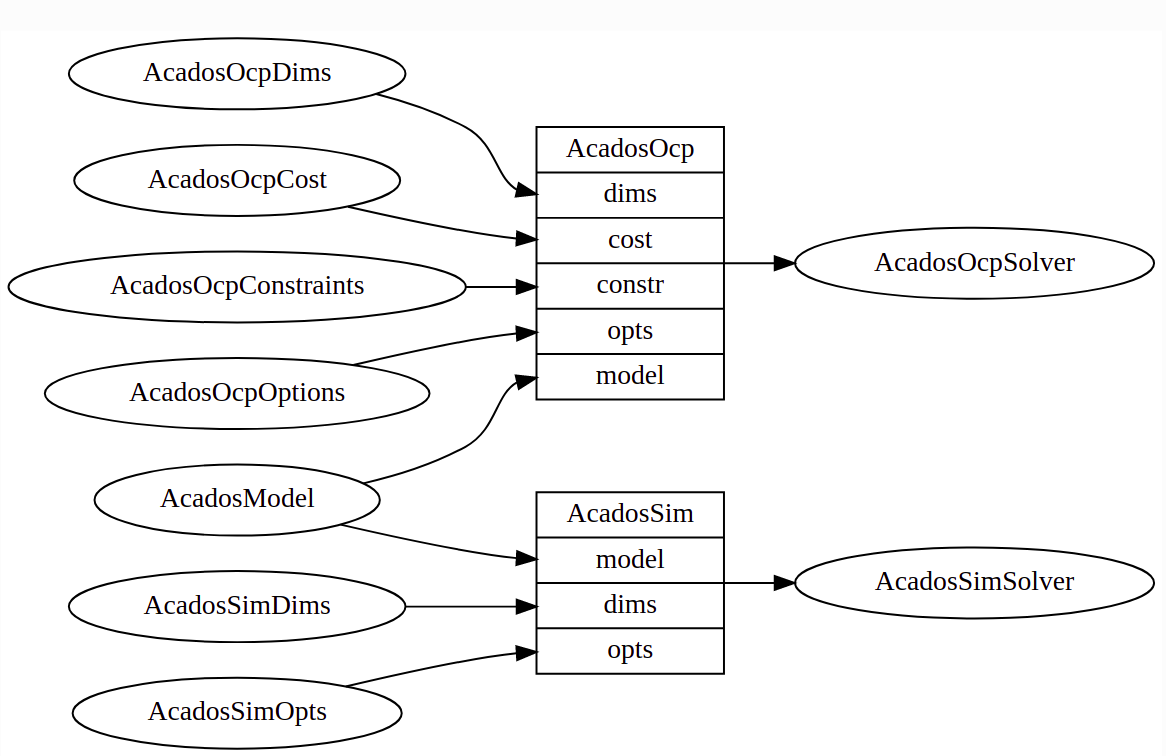
\includegraphics[width=0.8\textwidth]{Images/acados/python_interface.png}
 		\caption{Overview of the Python API classes in acados\protect\footnotemark}
 		\label{fig:python_interface}
 	\end{figure}
 		\footnotetext[6]{\tiny{\url{https://docs.acados.org/python_api/}}}
\end{frame}



\section{MPC Design}

\begin{frame}
	\frametitle{Assumptions used}
	\Fontvi
	
	Assumptions to considered when using the equations of motion in the planar and 3D case:
	
	\begin{itemize} % [<+->]
		\item Rigid structure.
		\item Symmetric structure.
		\item CoG and origin of body-fixed frame coincide.
		\item Propellers are rigid.
		\item Thrust and drag are proportional to the square of the velocity of the propeller.
	\end{itemize}

\end{frame}


\begin{frame}
	\frametitle{Equations of Motion of the Planar Quadrotor case}
	\Fontvi
	
	The equations of motion of the planar quadrotor are:
	\begin{equation}\label{dynamics_planar_quadrotor}
 \begin{cases} 
       \ddot{y} = - \frac{u_1}{m} \sin{\phi} \\
       \ddot{z} = - g + \frac{u_1}{m} \cos{\phi} \\
       \ddot{\phi} = \frac{u_2}{I_{xx}} \\
   \end{cases}
\end{equation}

With: 

\begin{itemize}
	\item $u_1$: Total thrust applied on the planar quadrotor.
	\item $u_2$: Torque applied by the planar quadrotor along the x-axis.
\end{itemize}

\end{frame}



\begin{frame}
	\frametitle{Equations of Motion of the 3D Quadrotor case}
	\Fontvi
	
	The equations of motion of a quadrotor:
	$$
	\text{Translational model: }\left\{
	\begin{array}{ll}				
		\dot{\bm{p}_i} &= \bm{v}_i \\
		\dot{\bm{v}_i} &= 
		\frac{T}{m} 
		\begin{bmatrix}
		2 (q_w q_y + q_x q_z) \\
		2 (q_y q_z - q_w q_x) \\
		1 - 2(q_x^2 + q_y^2 ) \\
		\end{bmatrix} + \bm{g} \\	
	\end{array}
	\right.
	$$
	$$
	\text{Rotational model: }\left\{
	\begin{array}{ll}		
		\dot{\bm{q}_i} & = \frac{1}{2}
		\begin{bmatrix}
		0 \\
		\bm{\omega}_i \\
		\end{bmatrix} \otimes \bm{q}_i \\
		\dot{\bm{\omega}_i} &= \bm{I}_i^{-1} \bm{\tau}_i - \bm{I}_i^{-1} (\bm{\omega}_i \times \bm{I}_i \bm{\omega}_i)
		\end{array}
		\right.
	$$
		\end{frame}

\begin{frame}
	\frametitle{Equations of Motion of the 3D Quadrotor case}
	\Fontvi
	
	However, the MPC controller will not account for all of the equations (Non-centralized MPC):
	$$
		\text{Treated by the MPC: }\left\{
		\begin{array}{lll}				
			\dot{\bm{p}_i} &= \bm{v}_i \\
			\dot{\bm{v}_i} &= 
			\frac{T}{m} 
			\begin{bmatrix}
				2 (q_w q_y + q_x q_z) \\
				2 (q_y q_z - q_w q_x) \\
				1 - 2(q_x^2 + q_y^2 ) \\
			\end{bmatrix} + \bm{g} \\			
			\dot{\bm{q}_i} & = \frac{1}{2}
			\begin{bmatrix}
				0 \\
				\bm{\omega}_i \\
			\end{bmatrix} \otimes \bm{q}_i \\
		\end{array}
		\right.
	$$
	$$
			\text{Treated by the L.L. controller: }\left\{
			\begin{array}{l}	
				\dot{\bm{\omega}_i} = \bm{I}_i^{-1} \bm{\tau}_i - \bm{I}_i^{-1} (\bm{\omega}_i \times \bm{I}_i \bm{\omega}_i)
			\end{array}
			\right.
	$$

	\begin{alertblock}{Remark}
		\begin{itemize} %[<+->]
			\item A low level controller is assumed to exist to map the angular rates inputs $\bm{\omega}$ to the required torques $\bm{\tau}$. 
			\item The equations above do not represent the complete model of the system.
			\begin{itemize}
				\item However, they are sufficient to control the quadrotor.
			\end{itemize}
		\end{itemize}
	\end{alertblock}						
				
\end{frame}


\begin{frame}
	\frametitle{Parameters of the Crazyflie 2.1}
	\Fontvi
	
    \begin{columns}
        \begin{column}{0.4\textwidth}
            \begin{figure}
                \centering
                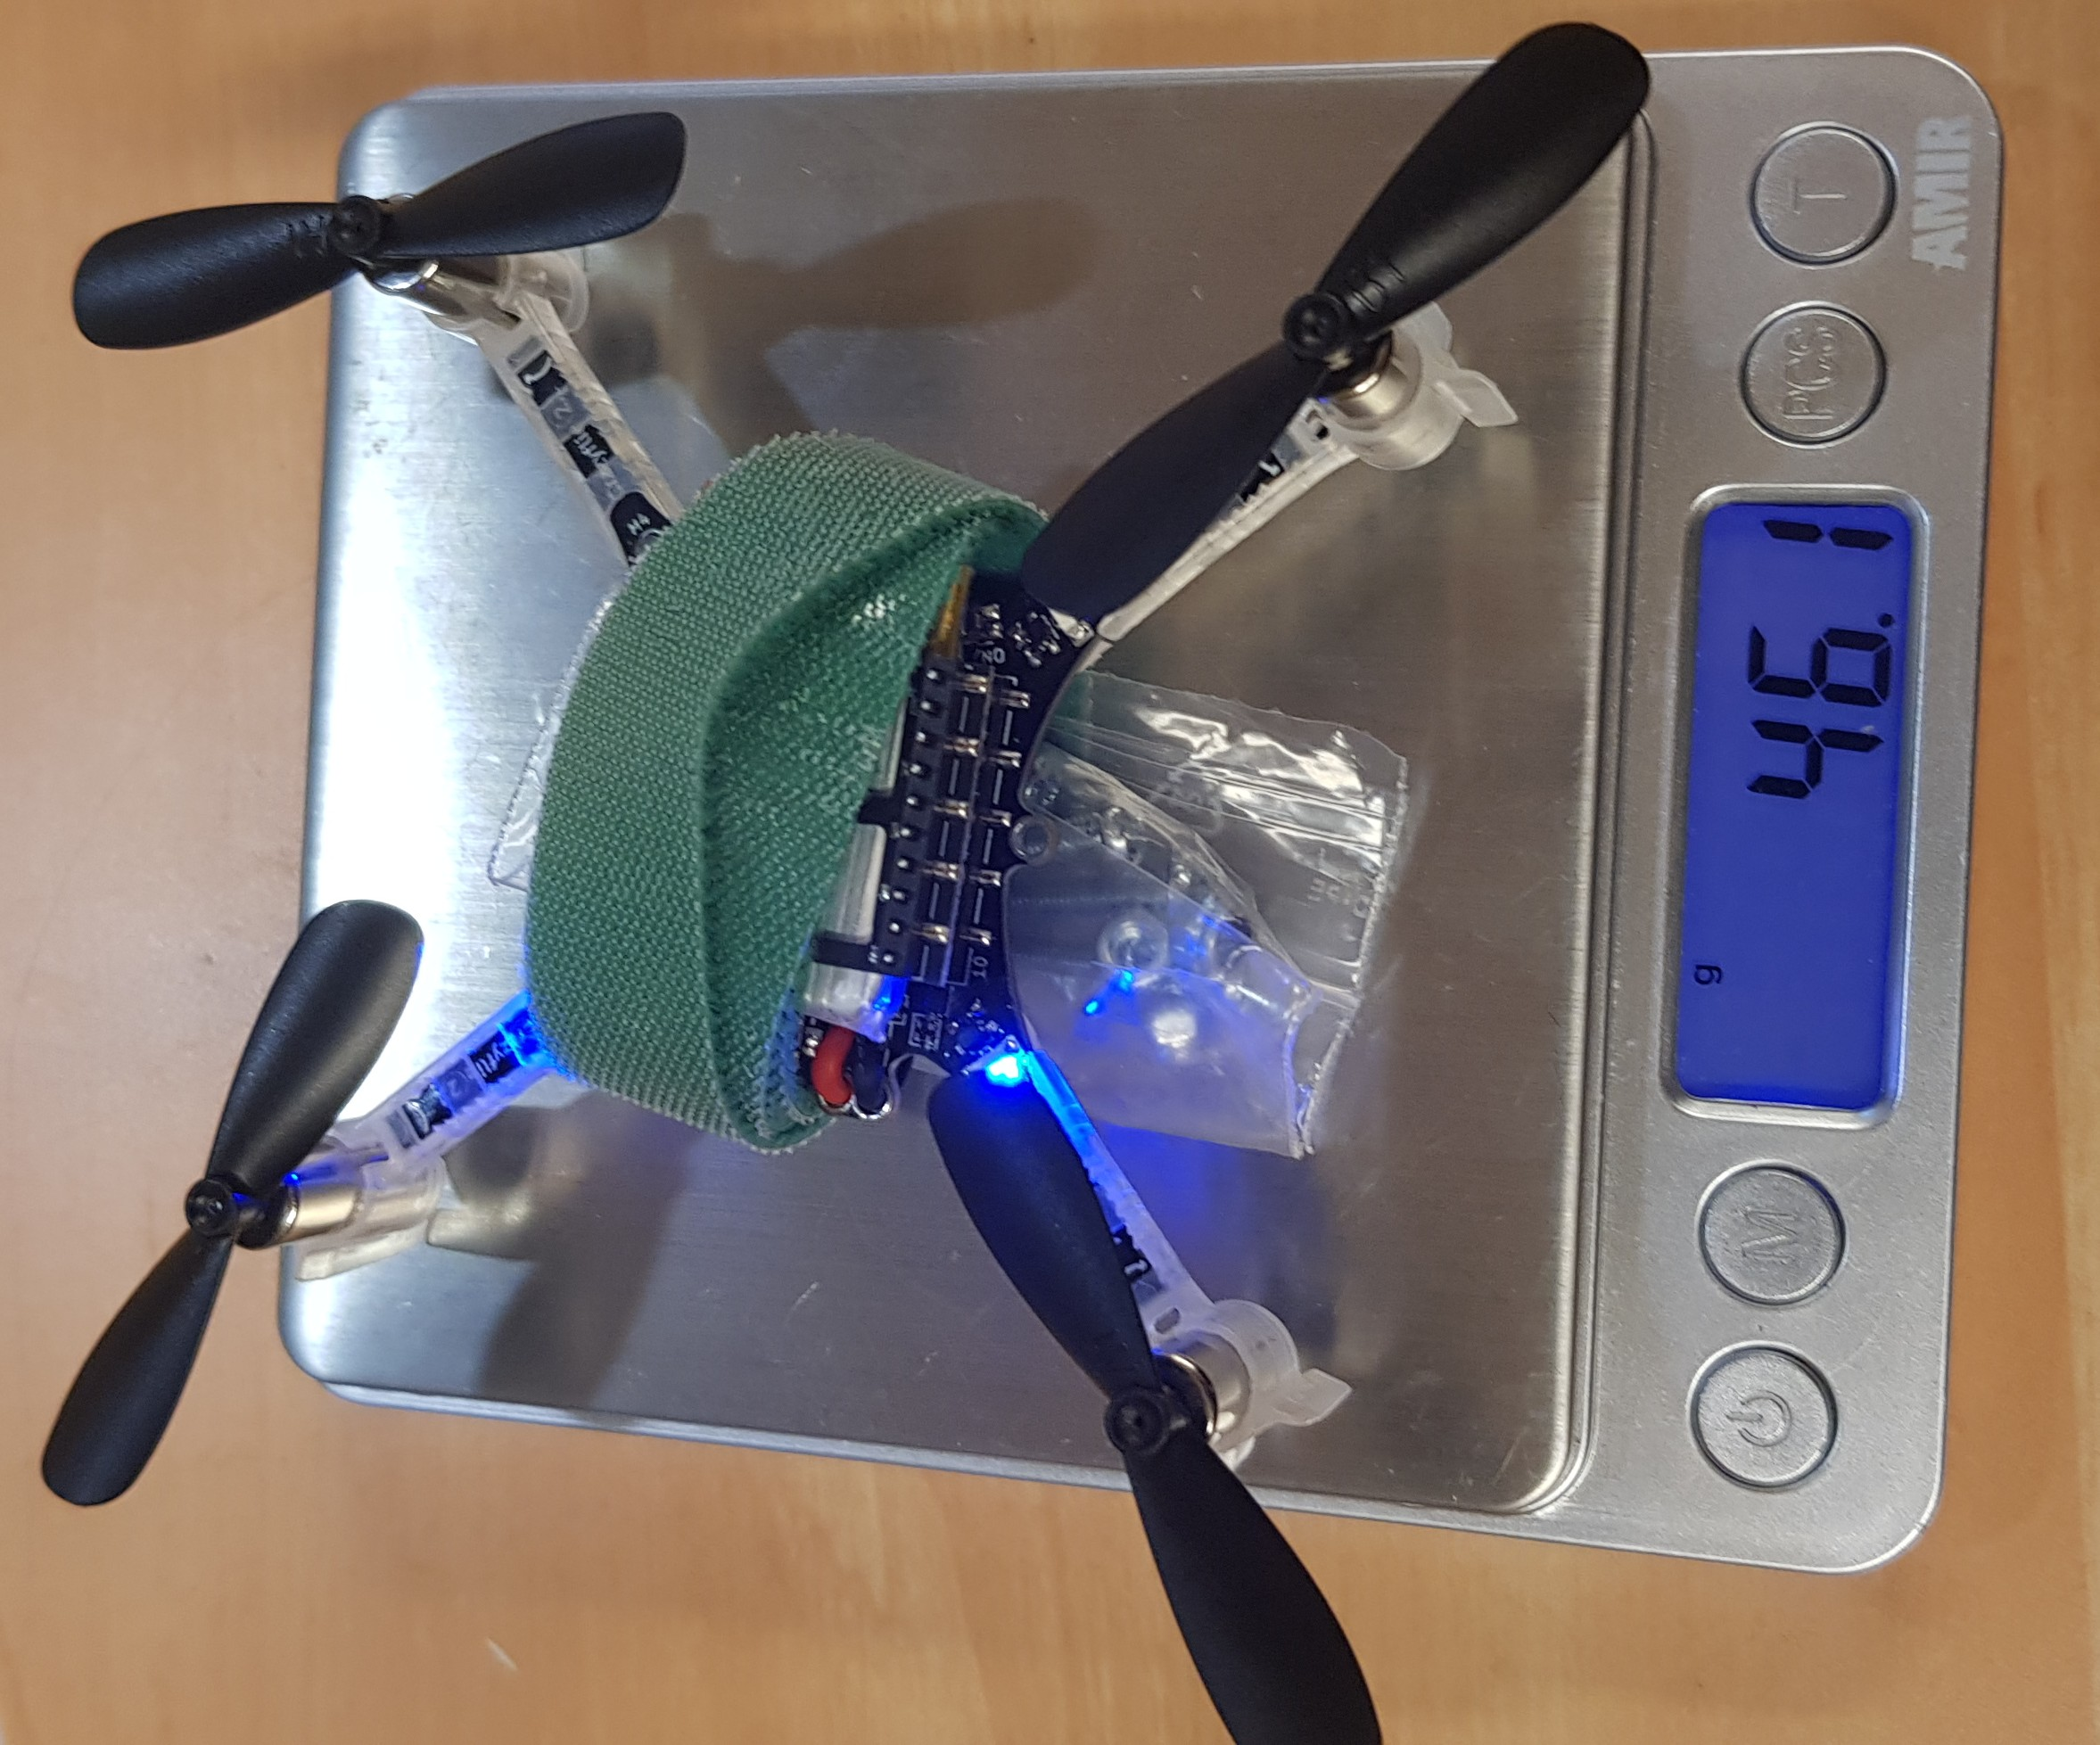
\includegraphics[height=0.5\textheight, angle =-90]{Images/crazyflie/max_thrust.jpg}
                \caption{Crazyflie 2.1 with added mass}
            \end{figure}
        \end{column}
        \begin{column}{0.6\textwidth}
            \begin{itemize}
                \item $m_{no\_load} =  29.5 g $
                \item $m_{with\_load} = 47 g $
                \item $T_{max}^{actual} = (47 \times 10^{-3} kg) 9.81 \frac{m}{s^2} = 0.46N $
				\item $I_{xx}$ = $1.657171 \times 10^{-5}  kg.m^2$
				\item $I_{yy}$ = $1.657171 \times 10^{-5}  kg.m^2$
				\item $I_{zz}$ = $2.9261652 \times 10^{-5} kg.m^2$
				\item $L = 0.046m$            
            \end{itemize}
        \end{column}
    \end{columns}
\end{frame}


\begin{frame}
	\frametitle{MPC for the Planar Quadrotor case}
	
	For the planar quadrotor case:
	
	\begin{equation}\label{mpc_optimization_problem_planar_quadrotor}
\begin{aligned}
            \min_{x,u} \quad & \frac{1}{2}\|\bm{V}_x \bm{x} + \bm{V}_u \bm{u} + \bm{V}_z \bm{z} - \bm{y}_{ref}\|^2_{\bm{W}} + \frac{1}{2}\|\bm{V}_x^e \bm{x} - \bm{y}_{ref}^e \|^2_{\bm{W}_e} \\
            \textrm{s.t.} \quad & f(\bm{x},\bm{u}):\text{dynamics} \\
             0 &\leq u_1 \leq u_{1_{max}} \\
             - u_{2_{max}} &\leq u_2 \leq u_{2_{max}}
        \end{aligned}
\end{equation}
with: 
\begin{multicols}{3}
\begin{itemize}
	\item $\bm{V}_x \in \mathbb{R}^{n_y \times n_x}$
	\item $\bm{V}_u \in \mathbb{R}^{n_y \times n_u}$ 
	\item $\bm{V}_z \in \mathbb{R}^{n_y \times n_z}$
	\item $\bm{V}_x^e \in \mathbb{R}^{n_{ye}\times n_x}$
\end{itemize}
\columnbreak
\begin{itemize}
	\item $\bm{y}_{ref} \in \mathbb{R}^{n_y}$
	\item $\bm{y}_{ref_e} \in \mathbb{R}^{n_{y_e}}$
	\item $\bm{W} \in \mathbb{R}^{n_y \times n_y}$
	\item $\bm{W}_e \in \mathbb{R}^{n_{y_e} \times n_{y_e}}$
\end{itemize}
\columnbreak
\begin{itemize}
	\item $\bm{Q},\bm{Q}_e \in \mathbb{R}^{n_x \times n_x}$
	\item $\bm{R} \in \mathbb{R}^{n_u \times n_u}$
	\item $\bm{W} = diag(\bm{Q},\bm{R}) $
	\item $\bm{W}_e = \bm{Q}_e $
\end{itemize}
\end{multicols}
\end{frame}

\begin{frame}
	\frametitle{MPC for the Planar Quadrotor case}
	
    \begin{columns}
        \begin{column}{0.5\textwidth}
            The state space variables:
            \begin{equation}
                \bm{x} = [y, z, \phi, v_y, v_z, \dot{\phi}]^{\intercal}
            \end{equation}
            The state evolves according to: 
            \begin{equation}
                \dot{y} = v_y
            \end{equation}
            \begin{equation}
                \dot{z} = v_z
            \end{equation}
            \begin{equation}
                \dot{\phi} = \dot{\phi}
            \end{equation}
            \begin{equation}
                \dot{v}_y = - \frac{u_1}{m} \sin(\phi)
            \end{equation}
            \begin{equation}
                \dot{v}_z = - g + \frac{u_1}{m} \cos(\phi)
            \end{equation}
            \begin{equation}
                \ddot{\phi} = \frac{u_2}{I_{xx}}
            \end{equation}   
        \end{column}
        \begin{column}{0.5\textwidth}
            Control inputs:
            $\bm{u} = [u_1, u_2]^{\intercal}$\\
            Initial condition: \\
            $\bm{x}_0 = [ y_0, z_0, \phi_0, v_{y_0}, v_{z_0}, \ddot{\phi}_0]^{\intercal}$\\
            \vfill
            Desired states: \\
            $\bm{x}_d = [y_d,z_d,\phi_d, v_{y_d},v_{z_d},\ddot{\phi}_d]^{\intercal}$
            \vfill
            MPC parameters: 
            \begin{itemize}
                \item $N = 100$
                \item $T_f = 1s$
                % \item $T_{sim} = 20$
            \end{itemize}
            Maximum thrust and torque:
            \begin{itemize}
                \item $u_{1_{max}} = 0.9 \bigg(\frac{0.46 N }{2}\bigg)$
                \item $u_{2_{max}} = 0.1 \bigg(\frac{1}{2} u_{1_{max}} L \bigg)$ 
            \end{itemize}
        \end{column}
    \end{columns}
\end{frame}


\begin{frame}
	\frametitle{MPC for the 3D Quadrotor case}
	
	For the 3D quadrotor case:
	\begin{equation}\label{mpc_optimization_problem_3d_quadrotor}
\begin{aligned}
            \min_{x,u} \quad & \frac{1}{2}\|\bm{V}_x \bm{x} + \bm{V}_u \bm{u} + \bm{V}_z \bm{z} - \bm{y}_{ref}\|^2_{\bm{W}} + \frac{1}{2}\|\bm{V}_x^e \bm{x} - \bm{y}_{ref}^e \|^2_{\bm{W}_e} \\
            \textrm{s.t.} \quad & f(\bm{x},\bm{u}):\text{dynamics} \\
             0 &\leq T \leq T_{max} \\
             -4 \pi &\leq \omega_x, \omega_y, \omega_z \leq 4 \pi
        \end{aligned}
\end{equation}
with: 
\begin{multicols}{3}
\begin{itemize}
	\item $\bm{V}_x \in \mathbb{R}^{n_y \times n_x}$
	\item $\bm{V}_u \in \mathbb{R}^{n_y \times n_u}$ 
	\item $\bm{V}_z \in \mathbb{R}^{n_y \times n_z}$
	\item $\bm{V}_x^e \in \mathbb{R}^{n_{ye}\times n_x}$
\end{itemize}
\columnbreak
\begin{itemize}
	\item $\bm{y}_{ref} \in \mathbb{R}^{n_y}$
	\item $\bm{y}_{ref_e} \in \mathbb{R}^{n_{y_e}}$
	\item $\bm{W} \in \mathbb{R}^{n_y \times n_y}$
	\item $\bm{W}_e \in \mathbb{R}^{n_{y_e} \times n_{y_e}}$
\end{itemize}
\columnbreak
\begin{itemize}
	\item $\bm{Q},\bm{Q}_e \in \mathbb{R}^{n_x \times n_x}$
	\item $\bm{R} \in \mathbb{R}^{n_u \times n_u}$
	\item $\bm{W} = diag(\bm{Q},\bm{R}) $
	\item $\bm{W}_e = \bm{Q}_e $
\end{itemize}
\end{multicols}
	
\end{frame}

\begin{frame}[t]{Centralized MPC}
    The state space variables:
    \begin{equation}
        \bm{x}= [x, y, z, q_w, q_x, q_y, q_z, v_x, v_y, v_z, ]^{\intercal}
    \end{equation} 
    \vfill
    Control inputs: 
    $\bm{u} = [T, \omega_x, \omega_y, \omega_z]^{\intercal}$\\
    \vfill
    Initial condition: \\
    $\bm{x}_0 = [ x_0, y_0, z_0, q_{w_0}, q_{x_0}, q_{y_0}, q_{z_0}, v_{x_0}, v_{y_0}, v_{z_0}]^{\intercal}$\\
    \vfill
    Desired states: \\
    $\bm{x}_d = [x_d,y_d,z_d, q_{w_d}, q_{x_d}, q_{y_d}, q_{z_d}, v_{x_d}, v_{y_d}, v_{z_d}]^{\intercal}$
    
    \vfill
    MPC parameters: 
    \begin{itemize}
        \item $N = 100$
        \item $T_s = 1s$
        % \item $T_{hover} = 2$s
        % \item $T_{traj}: \text{depends on the trajectory}$
    \end{itemize}
    
    Maximum thrust and torque:
    	\begin{itemize}
        	\item $T_{max} = 0.9 (0.46 N)$
        \end{itemize}
\end{frame}

\begin{frame}[t]{Centralized MPC} \vspace{4pt}
    The states evolve according to:
    \begin{columns}
        \begin{column}{0.5\textwidth}
            \begin{equation*}
                \dot{x} = v_x
            \end{equation*}
            \begin{equation*}
                \dot{y} = v_y
            \end{equation*}
            \begin{equation*}
                \dot{z} = v_z
            \end{equation*}
            \begin{equation*}
                \dot{q}_w=\frac{1}{2}( - w_x q_x - w_y q_y - w_z q_z)
            \end{equation*}
            \begin{equation*}
                \dot{q}_x=\frac{1}{2}( w_x q_w + w_z q_y - w_y q_z)
            \end{equation*}
        \end{column}
        \begin{column}{0.5\textwidth}
            \begin{equation*}
                \dot{q}_y=\frac{1}{2}( w_y q_w - w_z q_x + w_x q_z)
            \end{equation*}
            \begin{equation*}
                \dot{q}_z=\frac{1}{2}( w_z q_w + w_y q_x - w_x q_y)
            \end{equation*}
            \begin{equation*}
                \dot{v}_x = 2( q_w q_y + q_x q_z )\frac{T}{m}
            \end{equation*}
            \begin{equation*}
                \dot{v}_y = 2(q_y q_z - q_w q_x )\frac{T}{m}
            \end{equation*}
            \begin{equation*}
                \dot{v}_z = ( 1 - 2 q_x^2 - 2 q_y^2 )\frac{T}{m} - g
            \end{equation*}
        \end{column}
    \end{columns}
\end{frame}


\section{Flip Trajectory Generation}

\begin{frame}
	\frametitle{Physics of a Quadrotor Flip}
	\Fontvi
	
	The physics of a quadrotor flip can be divided into 4 parts:

	\begin{itemize}% [<+->]
		\item \textbf{Climb phase}: Maximum vertical acceleration is applied.
		\item \textbf{Multi-flip phase}: It ends when the desired $2n\pi$ are achieved.
		\item \textbf{Descent phase}: Maximum thrust for descent compensation.
		\item \textbf{Re-stabilization}: Altitude regulation to desired value. 
	\end{itemize}

	\begin{figure}[h]
		\centering
		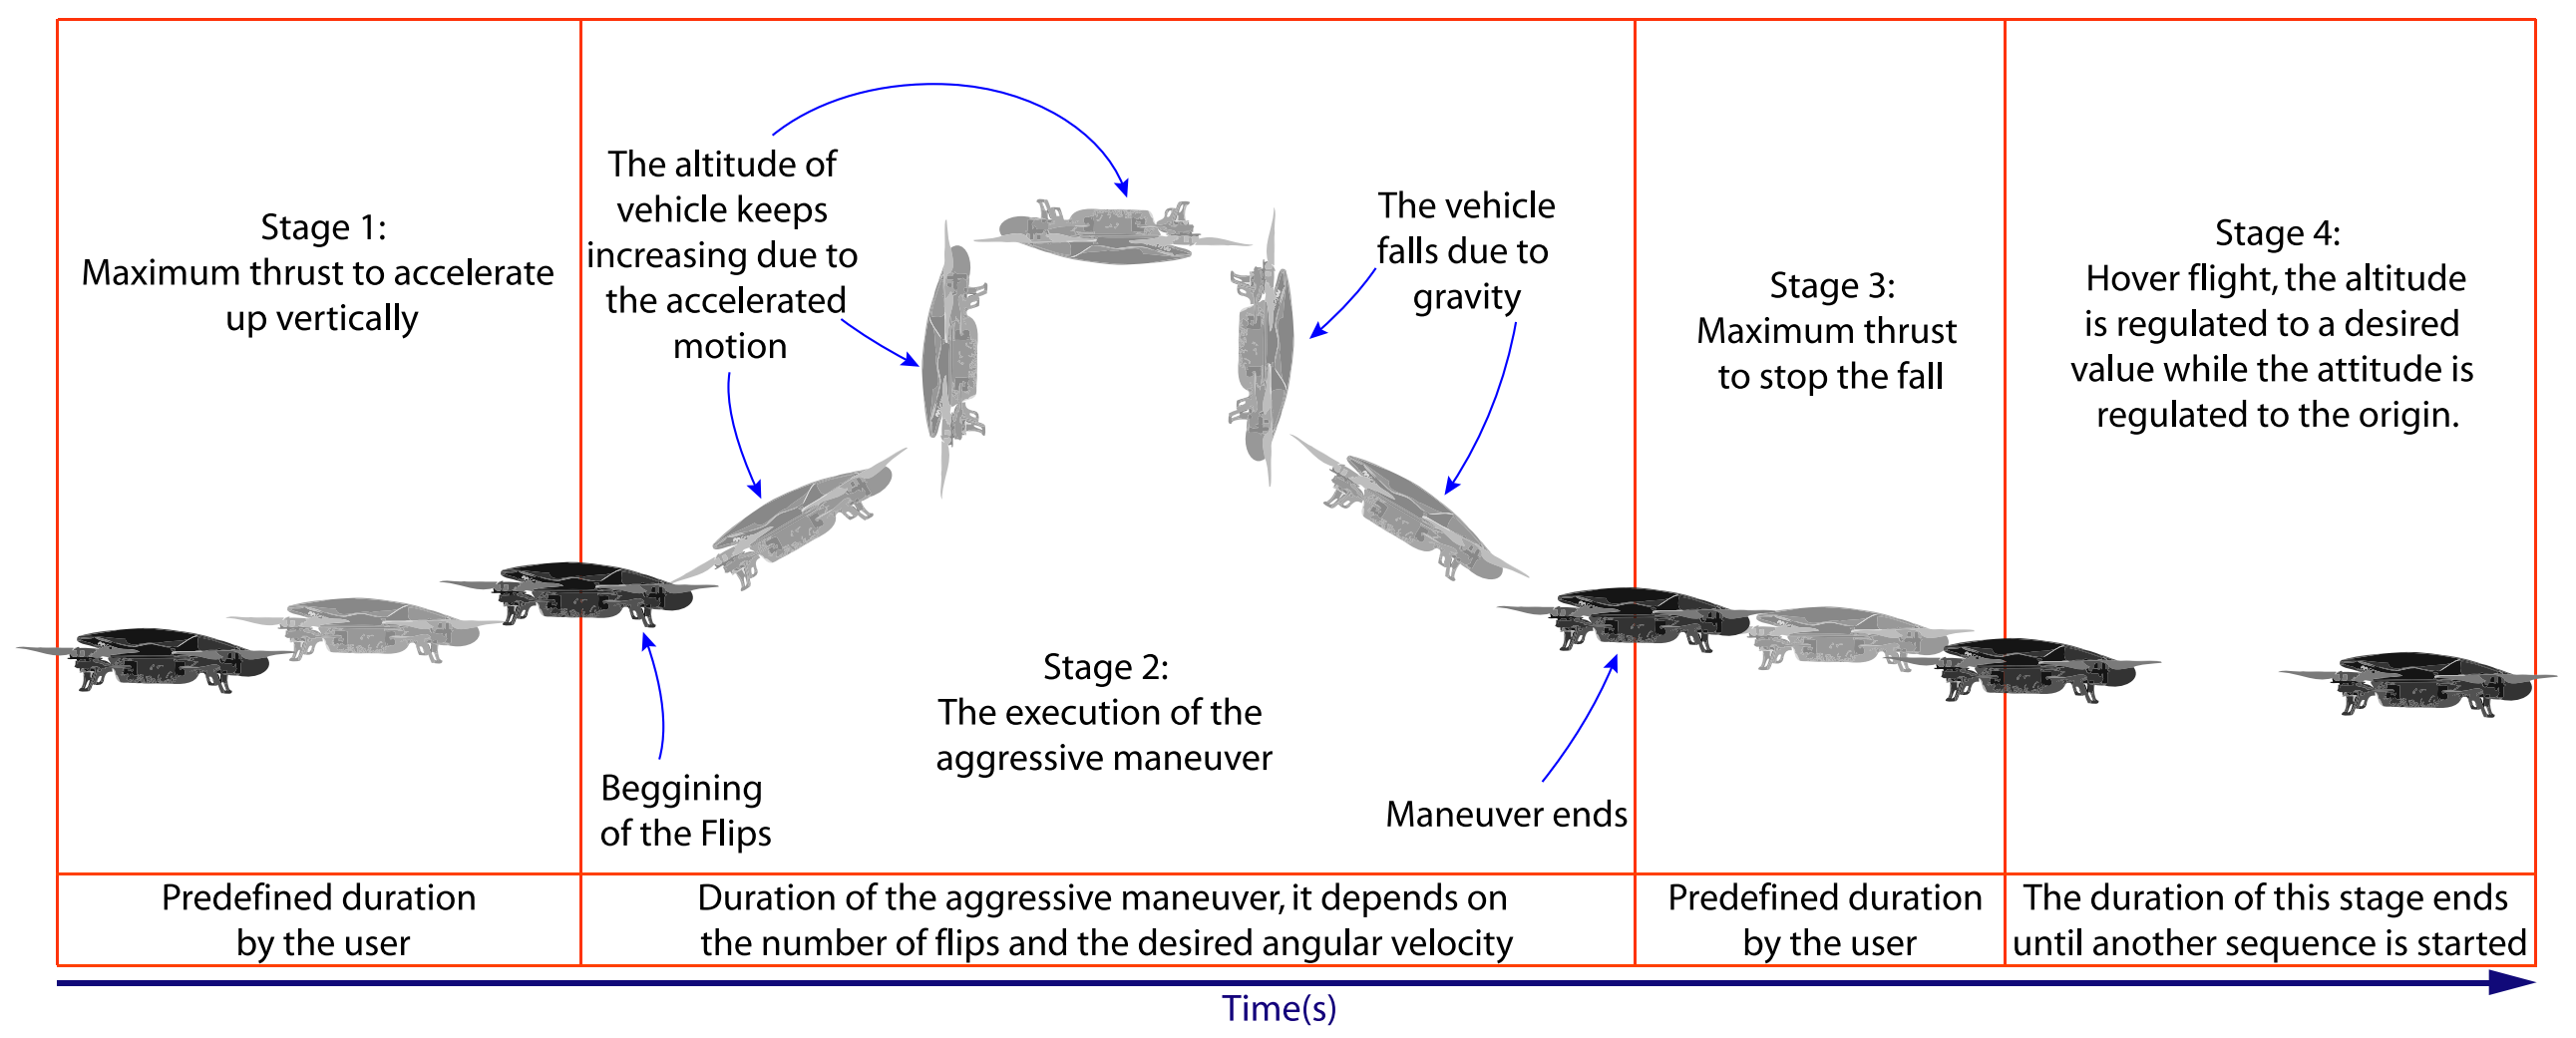
\includegraphics[width=0.8\textwidth]{Images/Flip/Physics}
		\caption{The phases needed for performing multi-flip maneuvers \protect\footnotemark}
		\label{flipping_physics}
	\end{figure}

\footnotetext[7]{\tiny{Nonlinear ellipsoid based attitude control for aggressive trajectories in a quadrotor: closed-loop multiflips implementation, 2018, F. {Oliva-Palomo} et al.}}

\end{frame}

\begin{frame}
	\frametitle{Dynamic Criterion of a Planar Quadrotor}
	\Fontvi
	
	The dynamic criterion of a planar quadrotor is\protect\footnotemark:
	
	\begin{equation}\label{dynamics_criterion_equation}
	\ddot{y} \cos \phi + (\ddot{z} + g) \sin \phi = 0
	\end{equation}


	\begin{itemize}
		\item It represents the dynamics constraints that must be satisfied to track a trajectory.
	\end{itemize}

	\vfill	
	To design dynamically feasible flip trajectories:
	
	\begin{itemize}
		\item The trajectories along $z$ and $\phi$ will be generated using polynomials of order 9.
		\item The trajectory along $y$ will then be computed by integrating the dynamic criterion twice: 
		\begin{equation}
			y(t) = - \iint (\ddot{z} + g) \tan \phi dt dt
		\end{equation}
	\end{itemize}
	
	\footnotetext[8]{\tiny{Making aggressive maneuvers with drones thanks to parallel singularity crossing approaches, 2019, M. Orsingher}}

\end{frame}










































\begin{frame}{Introduction}
\begin{itemize}[<+->]
\item Some
\item Appearing
\item Bullets
\begin{itemize}
 \item With sub-bullets
\end{itemize}
\end{itemize} 
 \visible<+-> {
 \begin{center}
  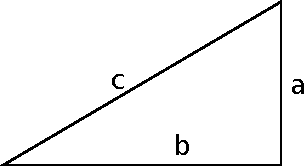
\includegraphics[width=.4\linewidth]{triangle1} \\
  And an appearing figure.
 \end{center}
 }
\end{frame}


\begin{frame}{Main content}
\begin{itemize}[<+>]
\item Some
\item Appearing
  \item And disappearing
\item Bullets
\begin{itemize}[<.>]
 \item With sub-bullets
\end{itemize}
\item That appear and disappear with their parent
\end{itemize}
\end{frame}



\begin{frame}{Main content}
\begin{enumerate}
\item Some	\vfill
\item Numbers
\begin{itemize}
 \item With sub-bullets
\end{itemize}\vfill
\item That appear and the same time\vfill
\item Nicely spaced on the slide
\end{enumerate}
\end{frame}


\begin{frame}{Citations}
 \begin{itemize}[<+->]
  \item Should be done with \textbackslash{fullcite}
  \begin{itemize}[<.->]
   \item \fullcite{pythm001}
  \end{itemize}\vfill
  \item You may also use \textbackslash{smallcite}
  \begin{itemize}[<.->]
   \item \smallcite{pythm001}
   \item It takes less space...
  \end{itemize}\vfill
  \item Check all imported references for:
  \begin{itemize}[<.->]
   \item Name / Journal name / year / editor (journals)
   \item Carefully check conference name (IEEEexplore)
  \end{itemize}
 \end{itemize}
\end{frame}

\begin{frame}{Equations}
\begin{itemize}[<+->]
  \item Have a number if used with \texttt{\textbackslash{begin}\{equation\}}
  \begin{equation}
  \forall \phi: \quad \cos ^2 \phi + \sin^2\phi = 1
  \end{equation}\vfill
  \item Do not have a number if used with \texttt{\textbackslash{begin}\{equation*\}}
    \begin{equation*}
  \forall a, b: \quad (a+b)^2 = a^2 + 2ab + b^2
  \end{equation*}
    \item Another useful environment is simply  \texttt{\textbackslash{begin}\{center\}}
    \begin{center}
    $\forall a, b: \quad (a-b)^2 = a^2 - 2ab + b^2$
    \end{center}
    \begin{itemize}[<+->]
    \item Probably more suited to slides as we use less equation references
  \end{itemize} \vfill\vfill   
  \item Can also be included in the text / bullets
  \begin{itemize}[<+->]
    \item $\forall \phi: \quad  (\cos\phi+\sin\phi)^2 = 2\cos\phi\sin\phi + 1$
  \end{itemize}
\end{itemize}
\end{frame}



\end{document}
